\chapter{User Interface}


\section{Design}
Das Projekt erhält eine möglichst einfach gehaltene Benutzeroberfläche. Durch die farbliche Trennung von Funktionen und fixen Bereichen für die Daten, soll die Oberfläche einfach und Intuitiv gestaltet werden. Zusätzlich wird die Oberfläche Responsive gestaltet, damit die Oberfläche an alle Geräte angepasst wird.

Es wurden Mock-ups anhand von einfachen Handskizzen erstellt, um das aussehen und die Funktionen der Benutzeroberfläche zu planen.

\section{Ansichten}
\subsection{Startseite}
Die Startseite zeigt dem Benutzer Hilfestellungen an und führt den Benutzer durch die ersten Schritte. Auf der Linken Seite befindet sich das Menu und eine Suche. Oben Rechts findet der Benutzer den Loginbereich und die Benutzerangaben.

Beim Menu gibt es statische, sowie dynamische Einträge. Der Discoveryeintrag ist ein dynamischer Eintrag und zeigt die Anzahl gefundenen Geräte an.
\begin{figure} [H]
	\begin{center}
	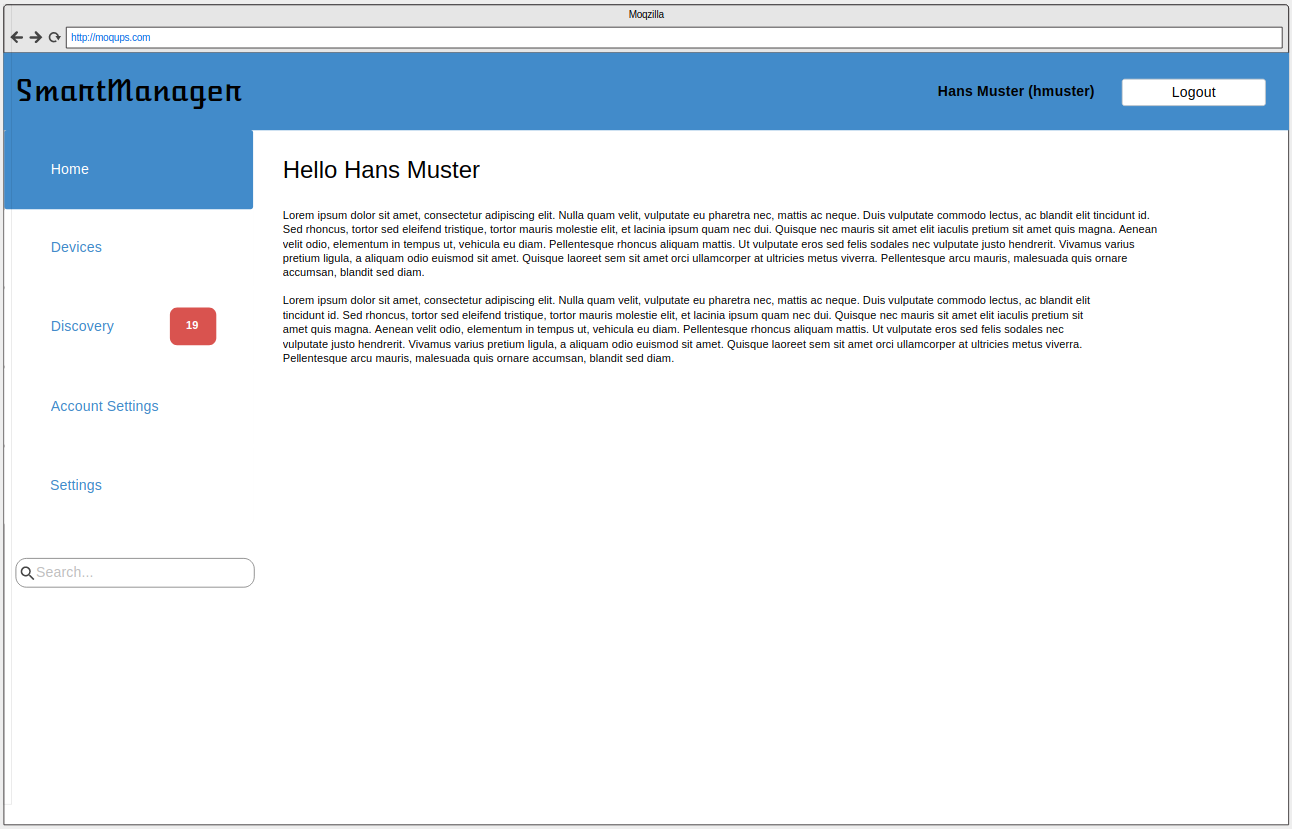
\includegraphics[width=0.80\textwidth]{images/home.PNG}
	\caption{\textbf{Startseite}}
	\label{Bild Referenz}
	\end{center}
\end{figure}


\subsection{Device List}
\begin{figure} [H]
	\begin{center}
	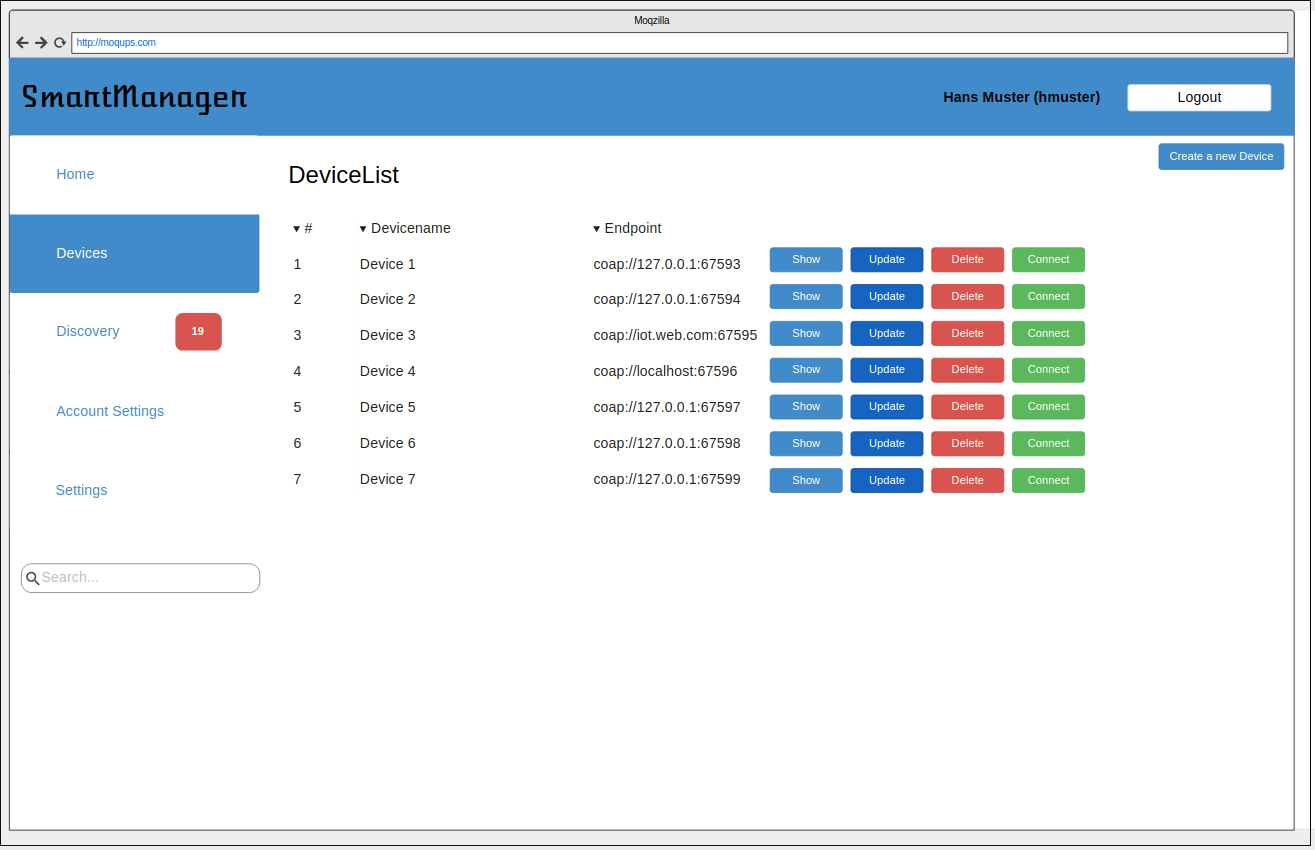
\includegraphics[width=0.80\textwidth]{images/devicelist.png}
	\caption{\textbf{Hauptansicht Menu}}
	\label{Device List}
	\end{center}
\end{figure}
In der Device Liste werden alle Devices angezeigt. Dazu wird zu jedem Device die jeweiligen Möglichkeiten als Button eingeblendet. So kann man ein Device betrachten, Anpassen, Löschen und sich mit dem Gerät verbinden. Zusätzlich werden die Daten, wie zum Beispiel Endpoint angezeigt.

Oben rechts befindet sich der Button, um weitere Devices zu erstellen.
\subsubsection{Buttons}

\begin{description}
\item [Show]
Verlinkt auf die \grqq{}Interface Selection\grqq{} Ansicht in welcher das aktive Interface zum Sniffen ausgewählt werden muss.
\item [Update]
Startet den Sessionfinder welche die aktiven Sessions in der Sessionliste auflistet.
\item [Delete]
Löscht die Liste der Sessions und startet die Aufzeichnung der Sessions neu.
\item [Connect]
Stopt den Sessionfinder und friert somit den Stand der Sessionliste ein.
\item [Create a newe Device]
Stopt den Sessionfinder und friert somit den Stand der Sessionliste ein.
\end{description}




\subsubsection{Create Device}
\begin{figure} [H]
	\begin{center}
	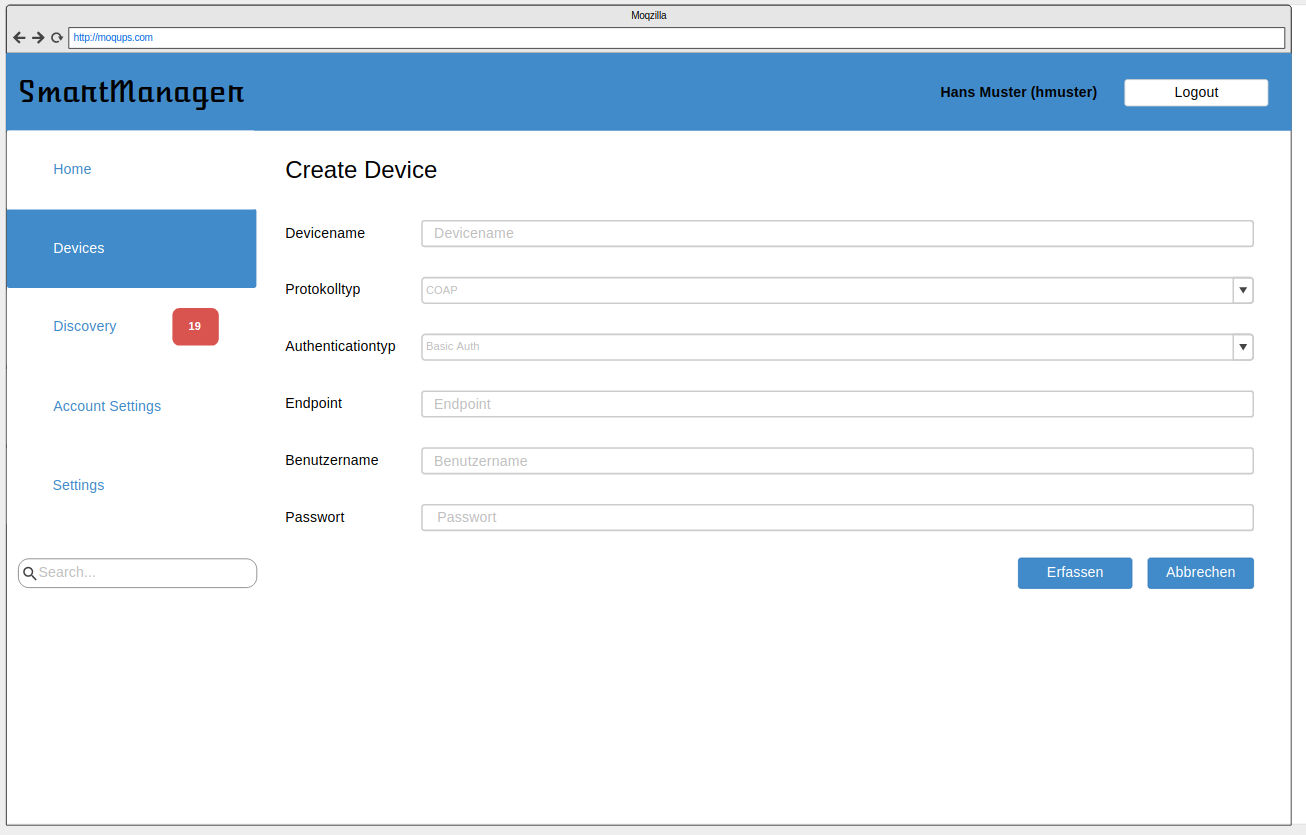
\includegraphics[width=0.80\textwidth]{images/createdevice.png}
	\caption{\textbf{Create Device}}
	\label{Hauptansicht Sessionfinder}
	\end{center}
\end{figure}
